%%----------------------------------------------------------------------
%%----------------------------------------------------------------------
\clearpage
\pagetitle{The Debacle on Caldor IV}

\begin{columns}

  \emph{The Debacle on Caldor IV} captures the last major thrusts at
  the conclusion of years of fighting over the planet.  All manner of
  allies and foes have come together to fight for whatever spoils
  Caldor IV may yield.

  \missionheading{Goals}

  With new, credible information confirming its existence having been
  unearthed recently, the Legions of Discord have formed an uneasy
  alliance seeking \emph{The Scythe of Unbound Light}, a war machine
  of incredible power believed to be still buried amid the planet's
  vast fields of rubble and dunes from its eons of strife.

  The Forces of Order are simply trying to extricate themselves from a
  rapidly worsening quagmire.  Originally the Mechanicum came to the
  planet in search of \emph{The Scythe}, but by this point only fools
  believe it still exists or ever did.  Magos Ferdinand, head of Mars'
  expedition, is such a fool and refused to evacuate until too late.
  Preparations are now underway to obliterate the planet, the
  situation having been deemed irrecoverable by sector governance.
  However, despite his foolish belief in ancient myths, the Magos'
  vast machine knowledge is too valuable to throw away easily. All
  effort necessary should be expended to retrieve him if at all
  possible before Exterminatus.

  Sensing opportunity amid the massive conflict, The Spoilers have
  come simply to smash and grab whatever they can while Order and
  Discord are occupied in a death struggle.  They would be happy to
  lay their claws on either \emph{The Scythe} or Magos Ferdinand.


  \missionheading{Continents}

  Caldor IV has three major continents over which the fighting has
  been concentrated:

  \begin{squishitemize}
  \item \textbf{Apollon:} Heaquarters of the Mechanicum, its primary
    forges, and more mysterious sites...

  \item \textbf{Hermea:} Home to the bulk of the world's civilian
    population in several miserable hive cities.

  \item \textbf{Juno:} Unreclaimed wastelands from the darkest periods
    of the past, not a place to go lightly.
  \end{squishitemize}

  Discord scryers believe \emph{The Scythe} is on Juno but will not
  stake their lives to it.  The precise location is necessary to
  retrieve it anyway.  Magos Ferdinand is assumed to be on Apollon,
  but his location has not been confirmed since the latest heavy
  fighting began.

\columnbreak
\begin{sidestory}{1.7in}{The Debacle on Caldor IV}
  Adept Kain's tentacled machine links withdrew slowly from the
  interface panels surrounding him. He had to cogitate, quietly,
  outside the noostream for a moment. Would this be his failure, or a
  brilliant recovery from failures made by those before him? Magos
  Ferdinand was a fool. This whole expedition had been a
  miscalculation from the start. From the poor research findings Kain
  had reviewed so far, he doubted their quarry had ever been more than
  a myth to begin with. And now the expedition's position had grown
  untenable, with incalculably valuable resources being thrown after a
  madman's quest. Slowly re-interfacing, he assented to the sector
  governor's request for exterminatus. Time to end this throne-cursed
  debacle.
\end{sidestory}

\missionheading{Terrain}

Each continent has a variety of areas represented by the various
tables available: City, industrial, wasteland, and so on.  There are
no specific campaign terrain requirements but players are able to
choose which boards they prefer to defend.  Tables should therefore be
set up in advance and have some distinct characteristics such as more
or less open sight lines and different concentrations of terrain
types.


\missionheading{Missions}

\emph{The Debacle on Caldor IV} is played out over the course of three
missions.  All players contest the same mission in each round.  Almost
any missions can be used, but a tournament ready mission pack is
included in this document following this section.

\missionheading{Campaign Setup}

Prepare two sets of three envelopes, one set for Order and the other
for Discord, each labelled for one of the continents on Caldor IV:
Apollon, Hermea, and Juno.  These envelopes capture the alliances'
search for \emph{The Scythe} and the Magos over each continent.

Print and cut out the Search Results cards at the end of this section.
Each card indicates the result of the alliance's searching over a
campaign round.  Some offer nothing, others reveal the target's
continent, and one yields their quarry's precise location.

As labelled on the cards, form two sets of four decks, one set each
for Order and Discord.  Shuffle each deck, keeping the cards facedown.
Randomly select a deck for both Order and Discord from their
respective sets and discard the others without revealing any cards.
Still keeping the cards facedown, for each one randomly select a
continent, e.g., by rolling a~D3.  Place the card into the appropriate
envelope for that alliance without revealing its content.

The search envelopes now contain clues to and the precise location of
each alliance's objective, randomly sprinkled across the continents.
Executed carefully, even the organizer(s) won't know where the targets
will be found and may participate as players in the campaign without
compromise.

\missionheading{Campaign Mechanics}

At the end of the three missions, Order and Discord have achieved
their campaign objective if they have discovered the precise location
of their target and hold the continent it is on.  The Spoilers achieve
their campaign objective if they know the precise location of either
\emph{The Scythe} or the Magos and hold that continent.  Note that the
precise location might be discovered on a different continent from the
target's actual location.  This reflects the worldwide search through
ruined libraries, hacked databanks, and captured individuals
eventually yielding the location, which must then be secured.  If a
precise location is found after the final round and the alliance has
control of that continent, they still achieve their campaign
objective.

\vfill
\noindent%
\begin{minipage}[t]{1.0\linewidth}\centering\small\it%
\fbox{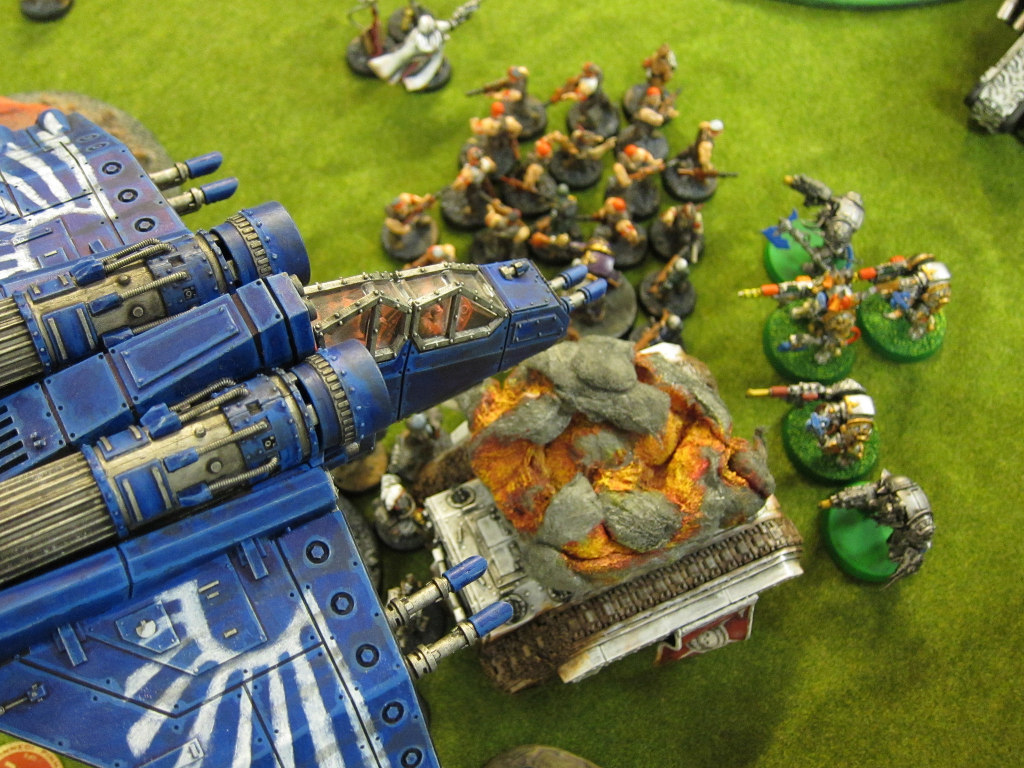
\includegraphics[width=(1.0\linewidth)]{pics/rob-flyer-sm}}\\
To the death!
\end{minipage}

\columnbreak

Following each round, Order and Discord draw and secretly keep a
search result from their respective envelopes for each continent they
control.  For each continent the Spoilers control they draw a search
result from the respective envelopes of both Order and Discord,
secretly record what they found, and put the card back in its
envelope.

Control of a continent is defined as the leader of the accumulated
sums for each alliance of victory points earned in matches held on
that continent.  In event of a tie, each of the tied alliances are
considered to have control.  If the Spoilers are among those tied,
they draw and return their results before the other alliances pull
from their envelopes.

\missionheading{Round Pairings}

For each match, players are paired with an opponent from another
alliance as best as possible given the number of players.  Teammates
should only battle if no other set of pairings is possible.  In that
rare case, their alliance earns the lesser of the two players' victory
points.  The players though each claim their respective victory points
toward the individual rankings.

First round pairings are randomly assigned across the alliances,
optionally applying a seeding to bias toward matching players of
similar ability.  Starting with the Legions of Discord, then the
Forces of Order, and then the Spoilers, the alliances alternate
choosing a pairing and assigning it to a continent.  The opposing
alliance then picks a table for that match.

In the second and third rounds, pairings are assigned randomly across
the alliances within win/loss brackets as best as possible.  No two
players may fight more than once, and opponents must be randomly
selected from within the closest possible win/loss brackets permitting
that, alternating shifts up and then down the brackets until a match
is possible.  Proceeding in order by the alliances' total
campaign-wide victory points and descending down the win/loss
brackets, the alliances alternate choosing a pairing and assigning it
to a continent.  The opposing alliance then responds with a table for
that match.



\missionheading{Victory!}

At the conclusion of \emph{The Debacle}, an alliance has won a
strategic victory if it achieved its campaign objective and no other
alliance did as well.  The alliance with the greatest sum total
victory points has won the tactical victory for the campaign.
Celebrate the victors, but prepare for the battles still ahead!

\end{columns}

\pagebreak
\squelchbackground

\newcommand{\searchalliance}{ALLIANCE}%
\newcommand{\searchresult}{No dice.}%
\newcommand{\searchstory}{You die painfully and alone.}%

\pgfmathsetmacro{\cardroundingradius}{2mm}
\pgfmathsetmacro{\striproundingradius}{1mm}
\pgfmathsetmacro{\ruleheight}{0.1}
\pgfmathsetmacro{\stripwidth}{1.1}
\pgfmathsetmacro{\stripheight}{1.1}
\pgfmathsetmacro{\strippadding}{0.1}
\pgfmathsetmacro{\textpadding}{0.3}

\pgfmathsetmacro{\searchcardwidth}{6}
\pgfmathsetmacro{\searchcardheight}{4.5}

\newcommand{\searchstripcolor}{black}
\newcommand{\searchstripfontsize}{}
\newcommand{\searchcaptionfontsize}{\footnotesize}
\newcommand{\searchtextfontsize}{}

\newcommand{\searchstriptext}%
  {\raisebox{-4pt}{\includegraphics[width=0.6cm]{icon-skull}} \hspace{0.25em} \searchalliance}


%%----------------------------------------------------------------------
%%----------------------------------------------------------------------
\newcommand{\drawsearchcard}{%
\begin{tikzpicture}%
  \clip (-0.05, -0.05) rectangle (\searchcardwidth+.05, \searchcardheight+.05);

  %%-- Draw the card back and outline
  \draw[rounded corners=\cardroundingradius,fill=white,draw=none] (0,0)
    rectangle (\searchcardwidth,\searchcardheight);
  \node[above left] at (\searchcardwidth+0.1, -0.1)
    {\includegraphics[height=4.2cm]{background-skull}};
  \draw[rounded corners=\cardroundingradius] (0,0) rectangle
    (\searchcardwidth,\searchcardheight);

  %%-- Draw the side strip
  \fill[\searchstripcolor,rounded corners=\striproundingradius]
    (\strippadding,\searchcardheight-\strippadding) rectangle
    (\searchcardwidth-\strippadding,\searchcardheight-\strippadding-\stripheight)
    node[right=-\searchcardwidth+\strippadding+\strippadding,yshift=16,white,font=\searchstripfontsize\fontfamily{ptm}\selectfont] {\raisebox{0pt}[13pt][5pt]{\vbox to -18pt{}} \searchstriptext};

  %%-- Draw the search result info lines
    \node[text width=(\searchcardwidth-\strippadding-\strippadding)*1cm,
          below right,inner sep=0] at
          (\strippadding,\searchcardheight-\stripheight-\strippadding-\strippadding-\textpadding)
    {\searchtextfontsize%
      \begin{minipage}{1.0\linewidth}\centering\sc\fontfamily{ptm}\selectfont
        \searchresult
      \end{minipage}
    };

    \node[text width=(\searchcardwidth-\strippadding-\strippadding)*1cm,
          above right,inner sep=0] at
          (\strippadding,\strippadding)
    {\searchcaptionfontsize%
      \begin{minipage}{1.0\linewidth}\centering\it
        \searchstory\raisebox{0pt}[9pt][3pt]{}
      \end{minipage}
    };

\end{tikzpicture}
}

\newcommand{\searchcard}[3]{%
\renewcommand{\searchalliance}{#1}%
\renewcommand{\searchresult}{#2}%
\renewcommand{\searchstory}{#3}%
\drawsearchcard%
}


\begin{landscape}
\vspace*{-15pt}

\noindent%
\searchcard{ORDER (1)}{Precise location:\\Apollon,\\Forge Prime.}{The
  Magos is bunkered deep in the bowels of Caldor IV's largest and
  oldest forge with his bodyguards.}\hfill%
\searchcard{ORDER (2)}{Precise location:\\Apollon,\\North
  Starport.}{Mechanicum forces are fighting to sustain a desperate
  holdout at the complex in hopes of evacuation.}\hfill%
\searchcard{ORDER (3)}{Precise location:\\Hermea,\\Hive
  Bahlus.}{Credible reports cite him cowering among the squalor and
  innumerable civilians of the lower hab blocks.}\hfill%
\searchcard{ORDER (4)}{Precise location:\\Juno,\\The Scar.}{The Magos
  is leading a frantic excavation at the bottom of one of Caldor IV's
  most unnatural features.}

\vfill

\noindent%
\searchcard{ORDER (1)}{Clue:\\Apollon.}{A planetary defense company\\
  reports seeing the Magos moving\\through Forge Praxus.}\hfill%
\searchcard{ORDER (2)}{Clue:\\Apollon.}{A small group of Skitarii,
  bodyguards of the Magos, were seen fighting on the outskirts of the
  North Starport.}\hfill%
\searchcard{ORDER (3)}{Clue:\\Hermea.}{Shuttle pilots report
  delivering the Magos' entourage to the continent at the onset of the
  recent fighting.}\hfill%
\searchcard{ORDER (4)}{Clue:\\Juno.}{A badly corrupted distress signal\\
  was received from one of the\\Magos' closest proteges.}

\vfill

\noindent%
\searchcard{ORDER (1)}{Clue:\\Apollon.}{Techmarines report the Magos
  recently logged into the noosphere from a terminal in Forge
  Maurus.}\hfill%
\searchcard{ORDER (2)}{Clue:\\Apollon.}{Reports indicate the Magos had
  ordered an orbital lifter prepared but it was damaged by ground
  fighting.}\hfill%
\searchcard{ORDER (3)}{Clue:\\Hermea.}{Official records indicate the
  Magos had scheduled an oversight meeting with one of the hive
  regents.}\hfill%
\searchcard{ORDER (4)}{Clue:\\Juno.}{The expedition's future dimming,
  of late the Magos had been obsessed with several sites in the
  wasteland.}

\vfill

\noindent%
\searchcard{ORDER}{No result.}{The Magos' personal logs are recovered
  but are woefully outdated and yield no hint of his location.}\hfill%
\searchcard{ORDER}{No result.}{Contact is made with a servant of the
  Magos but the line breaks before they can exchange any
  information.}\hfill%
\searchcard{ORDER}{No result.}{None of the senior adepts still alive
  and reachable have seen or heard from the Magos in quite some
  time.}\hfill%
\searchcard{TRASH}{Throw this placeholder card away, it is not used
  in the campaign.}{Thought for the day: Sacrifice is the strongest
  sign of devotion.}

\pagebreak

\noindent%
\searchcard{DISCORD (1)}{Precise location:\\Juno,\\.}{}\hfill%
\searchcard{DISCORD (2)}{Precise location:\\Juno,\\The Scar.}{}\hfill%
\searchcard{DISCORD (3)}{Precise location:\\Hermea,\\Hive
  Pargnosis.}{The mighty war engine slumbers deep in the lowest
  sub-foundation, quietly powering the entire hive.}\hfill%
\searchcard{DISCORD (4)}{Precise location:\\Apollon,\\Forge
  Prime.}{\emph{The Scythe} has lain unrecognized in the Mechanicum's
  vaults for decades, a colossal failure of imagination.}

\vfill

\noindent%
\searchcard{DISCORD (1)}{Clue:\\Juno.}{}\hfill%
\searchcard{DISCORD (2)}{Clue:\\Juno.}{Analysis of radiation patterns
  from metals unburied across the continent point toward a spectacular
  crash site.}\hfill%
\searchcard{DISCORD (3)}{Clue:\\Hermea.}{A beautiful tapestry
  allegorizes\\\emph{The Scythe} shielding Hermea's houses from
  staggering attacks.}\hfill%
\searchcard{DISCORD (4)}{Clue:\\Apollon.}{A faded manifest for
  sub-annex~42A of the original expedition complex lists wonders
  beyond belief.}


\vfill

\noindent%
\searchcard{DISCORD (1)}{Clue:\\Juno.}{}\hfill%
\searchcard{DISCORD (2)}{Clue:\\Juno.}{Something had to have torn
  those gouges out of the planet.}\hfill%
\searchcard{DISCORD (3)}{Clue:\\Hermea.}{Early texts chart the lineage
  of the population centers back to the survivors of the
  founding houses.}\hfill%
\searchcard{DISCORD (4)}{Clue:\\Apollon.}{An empty docking interface
  for \emph{The Scythe} is found, with Mechanicum extraction equipment
  nearby.}\hfill%

\vfill

\noindent%
\searchcard{DISCORD}{No result.}{The long sought-for vault's\\contents
  begin crumbling immediately upon exposure to atmosphere.}\hfill%
\searchcard{DISCORD}{No result.}{The ancient integrated librarian has
  only false beliefs and nonsense to share before you end his
  pain.}\hfill%
\searchcard{DISCORD}{No result.}{Your servants are imbeciles, fit for
  little more than scrap meat.}\hfill%
\searchcard{TRASH}{Throw this placeholder card away, it is not used
  in the campaign.}{Thought for the day:\\Sacrifice is best done by
  others.}

\end{landscape}

\pagebreak
\restorebackground


%\vfill
%\noindent%
%\begin{minipage}[t]{1.0\linewidth}\centering\small\it%
%\fbox{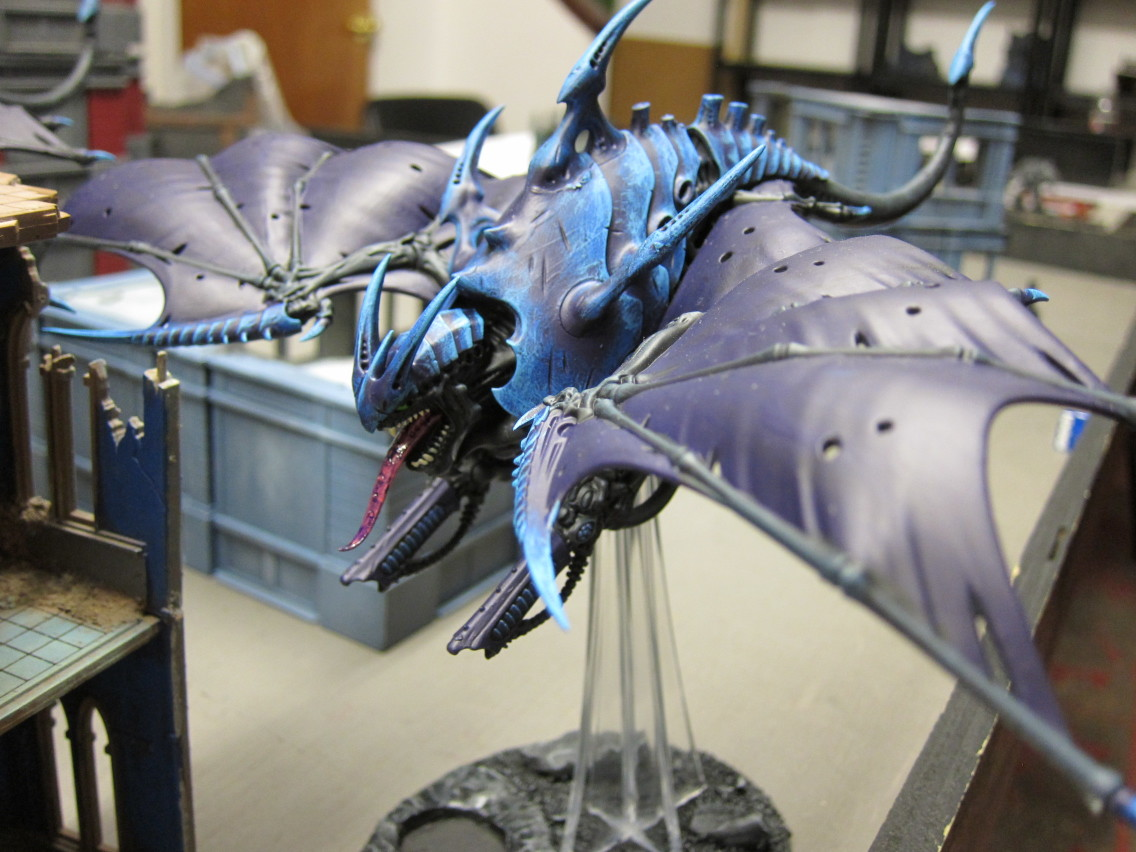
\includegraphics[width=(1.0\linewidth)]{pics/IMG_9230-sm}}\\
%Scour the skies!
%\end{minipage}
